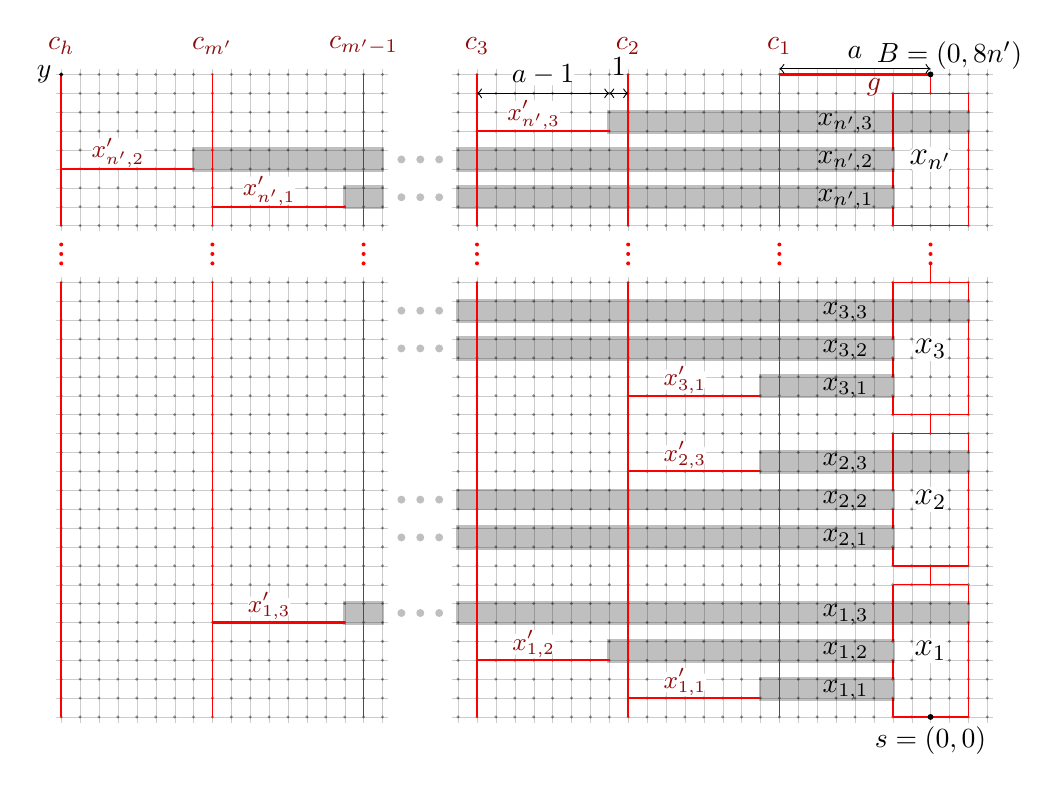
\begin{tikzpicture}[scale=0.24]
\definecolor{dred}{RGB}{143, 11, 11}
\def\wi{0.08}
\def\op{0.2}
\def\pts{2.5pt}

\foreach \x in {-25,...,3} {
\foreach \y in {0,...,23} {
\fill[black, opacity=0.4] (\x, \y) circle (\pts);
}
\draw[black, line width=\wi, opacity=\op] (\x, -0.3) -- (\x, 23.3);
}
\foreach \y in {0,...,23} {
\draw[black, line width=\wi, opacity=\op] (-25.3, \y) -- (3.3, \y);
\draw[black, line width=\wi, opacity=\op] (-46.3, \y) -- (-28.7, \y);
}
\foreach \y in {26,...,34} {
\draw[black, line width=\wi, opacity=\op] (-25.3, \y) -- (3.3, \y);
\draw[black, line width=\wi, opacity=\op] (-46.3, \y) -- (-28.7, \y);
}

\foreach \x in {-25,...,3} {
\foreach \y in {26,...,34} {
\fill[black, opacity=0.4] (\x, \y) circle (\pts);
}
\draw[black, line width=\wi, opacity=\op] (\x, 25.7) -- (\x, 34.3);
}


\foreach \x in {-46,...,-29} {
\foreach \y in {26,...,34} {
\fill[black, opacity=0.4] (\x, \y) circle (\pts);
}
\draw[black, line width=\wi, opacity=\op] (\x, 25.7) -- (\x, 34.3);

}
\foreach \x in {-46,...,-29} {
\foreach \y in {0,...,23} {
\fill[black, opacity=0.4] (\x, \y) circle (\pts);
}
\draw[black, line width=\wi, opacity=\op] (\x, -0.3) -- (\x, 23.3);
}
\draw[red, line width = 0.5669291340000001pt]   (-2, 0) -- (2, 0);
\draw[red, line width = 0.5669291340000001pt]   (-2, 0) -- (-2, 1);
\draw[red, line width = 0.5669291340000001pt]   (-2, 2) -- (-2, 3);
\draw[red, line width = 0.5669291340000001pt]   (-2, 4) -- (-2, 7);
\draw[red, line width = 0.5669291340000001pt]   (2, 0) -- (2, 5);
\draw[red, line width = 0.5669291340000001pt]   (2, 6) -- (2, 7);
\draw[red, line width = 0.5669291340000001pt]   (-2, 7) -- (2, 7);
\draw[red, line width = 0.5669291340000001pt]   (0, 7) -- (0, 8);
\node[fill=white, rounded corners, inner sep=1pt, outer sep=1pt] at (0, 3.5)  {\large $x_1$};
\draw[red, line width = 0.5669291340000001pt]   (-2, 8) -- (2, 8);
\draw[red, line width = 0.5669291340000001pt]   (-2, 8) -- (-2, 9);
\draw[red, line width = 0.5669291340000001pt]   (-2, 10) -- (-2, 11);
\draw[red, line width = 0.5669291340000001pt]   (-2, 12) -- (-2, 15);
\draw[red, line width = 0.5669291340000001pt]   (2, 8) -- (2, 13);
\draw[red, line width = 0.5669291340000001pt]   (2, 14) -- (2, 15);
\draw[red, line width = 0.5669291340000001pt]   (-2, 15) -- (2, 15);
\draw[red, line width = 0.5669291340000001pt]   (0, 15) -- (0, 16);
\node[fill=white, rounded corners, inner sep=1pt, outer sep=1pt] at (0, 11.5)  {\large $x_2$};
\draw[red, line width = 0.5669291340000001pt]   (-2, 16) -- (2, 16);
\draw[red, line width = 0.5669291340000001pt]   (-2, 16) -- (-2, 17);
\draw[red, line width = 0.5669291340000001pt]   (-2, 18) -- (-2, 19);
\draw[red, line width = 0.5669291340000001pt]   (-2, 20) -- (-2, 23);
\draw[red, line width = 0.5669291340000001pt]   (2, 16) -- (2, 21);
\draw[red, line width = 0.5669291340000001pt]   (2, 22) -- (2, 23);
\draw[red, line width = 0.5669291340000001pt]   (-2, 23) -- (2, 23);
\draw[red, line width = 0.5669291340000001pt]   (0, 23) -- (0, 24);
\node[fill=white, rounded corners, inner sep=1pt, outer sep=1pt] at (0, 19.5)  {\large$x_3$};
\draw[red, line width = 0.5669291340000001pt]   (-2, 26) -- (2, 26);
\draw[red, line width = 0.5669291340000001pt]   (-2, 26) -- (-2, 27);
\draw[red, line width = 0.5669291340000001pt]   (-2, 28) -- (-2, 29);
\draw[red, line width = 0.5669291340000001pt]   (-2, 30) -- (-2, 33);
\draw[red, line width = 0.5669291340000001pt]   (2, 26) -- (2, 31);
\draw[red, line width = 0.5669291340000001pt]   (2, 32) -- (2, 33);
\draw[red, line width = 0.5669291340000001pt]   (-2, 33) -- (2, 33);
\draw[red, line width = 0.5669291340000001pt]   (0, 33) -- (0, 34);
\node[fill=white, rounded corners, inner sep=1pt, outer sep=1pt] at (0, 29.5)  {\large $x_{n'}$};
\draw[black, line width = 8.736220474000001pt, opacity=0.25]   (-9.1, 1.5) -- (-1.9, 1.5);
\node at (-4.5, 1.4) { $x_{1, 1}$};
\draw[black, line width = 8.736220474000001pt, opacity=0.25]   (-17.1, 3.5) -- (-1.9, 3.5);
\node at (-4.5, 3.4) { $x_{1, 2}$};
\draw[black, line width = 8.736220474000001pt, opacity=0.25]   (-25.1, 5.5) -- (2.1, 5.5);
\node at (-4.5, 5.4) { $x_{1, 3}$};
\fill[black, opacity=0.25] (-26, 5.5) circle (6pt);
\fill[black, opacity=0.25] (-27, 5.5) circle (6pt);
\fill[black, opacity=0.25] (-28, 5.5) circle (6pt);
\draw[black, line width = 8.736220474000001pt, opacity=0.25]   (-31.1, 5.5) -- (-28.9, 5.5);
\draw[black, line width = 8.736220474000001pt, opacity=0.25]   (-25.1, 9.5) -- (-1.9, 9.5);
\node at (-4.5, 9.4) { $x_{2, 1}$};
\fill[black, opacity=0.25] (-26, 9.5) circle (6pt);
\fill[black, opacity=0.25] (-27, 9.5) circle (6pt);
\fill[black, opacity=0.25] (-28, 9.5) circle (6pt);
\draw[black, line width = 7.836220474000001pt, opacity=0.25]   (-25.1, 11.5) -- (-1.9, 11.5);
\node at (-4.5, 11.4) { $x_{2, 2}$};
\fill[black, opacity=0.25] (-26, 11.5) circle (6pt);
\fill[black, opacity=0.25] (-27, 11.5) circle (6pt);
\fill[black, opacity=0.25] (-28, 11.5) circle (6pt);
\draw[black, line width = 8.736220474000001pt, opacity=0.25]   (-9.1, 13.5) -- (2.1, 13.5);
\node at (-4.5, 13.4) { $x_{2, 3}$};
\draw[black, line width = 8.736220474000001pt, opacity=0.25]   (-9.1, 17.5) -- (-1.9, 17.5);
\node at (-4.5, 17.4) { $x_{3, 1}$};
\draw[black, line width = 8.736220474000001pt, opacity=0.25]   (-25.1, 19.5) -- (-1.9, 19.5);
\node at (-4.5, 19.4) { $x_{3, 2}$};
\fill[black, opacity=0.25] (-26, 19.5) circle (6pt);
\fill[black, opacity=0.25] (-27, 19.5) circle (6pt);
\fill[black, opacity=0.25] (-28, 19.5) circle (6pt);
\draw[black, line width = 8.736220474000001pt, opacity=0.25]   (-25.1, 21.5) -- (2.1, 21.5);
\node at (-4.5, 21.4) { $x_{3, 3}$};
\fill[black, opacity=0.25] (-26, 21.5) circle (6pt);
\fill[black, opacity=0.25] (-27, 21.5) circle (6pt);
\fill[black, opacity=0.25] (-28, 21.5) circle (6pt);
\draw[black, line width = 8.736220474000001pt, opacity=0.25]   (-25.1, 27.5) -- (-1.9, 27.5);
\node at (-4.5, 27.4) { $x_{n', 1}$};
\fill[black, opacity=0.25] (-26, 27.5) circle (6pt);
\fill[black, opacity=0.25] (-27, 27.5) circle (6pt);
\fill[black, opacity=0.25] (-28, 27.5) circle (6pt);
\draw[black, line width = 8.736220474000001pt, opacity=0.25]   (-25.1, 29.5) -- (-1.9, 29.5);
\node at (-4.5, 29.4) { $x_{n', 2}$};
\fill[black, opacity=0.25] (-26, 29.5) circle (6pt);
\fill[black, opacity=0.25] (-27, 29.5) circle (6pt);
\fill[black, opacity=0.25] (-28, 29.5) circle (6pt);
\draw[black, line width = 8.736220474000001pt, opacity=0.25]   (-17.1, 31.5) -- (2.1, 31.5);
\node at (-4.5, 31.4) { $x_{n', 3}$};
% \fill[black, opacity=0.25] (-26, 31.5) circle (6pt);
% \fill[black, opacity=0.25] (-27, 31.5) circle (6pt);
% \fill[black, opacity=0.25] (-28, 31.5) circle (6pt);
\draw[black, line width = 8.736220474000001pt, opacity=0.25]   (-31.1, 27.5) -- (-28.9, 27.5);
\draw[black, line width = 8.736220474000001pt, opacity=0.25]   (-39.1, 29.5) -- (-28.9, 29.5);
\node at (-8, 35.5)  {$\textcolor{dred}{c_1}$};
\draw[red, line width = 0.5669291340000001pt]   (-8, 0) -- (-8, 23);
\draw[red, line width = 0.5669291340000001pt]   (-8, 26) -- (-8, 34);
\fill[red] (-8, 24) circle (3pt);
\fill[red] (-8, 24.5) circle (3pt);
\fill[red] (-8, 25) circle (3pt);
\node at (-16, 35.5)  {$\textcolor{dred}{c_2}$};
\draw[red, line width = 0.5669291340000001pt]   (-16, 0) -- (-16, 23);
\draw[red, line width = 0.5669291340000001pt]   (-16, 26) -- (-16, 34);
\fill[red] (-16, 24) circle (3pt);
\fill[red] (-16, 24.5) circle (3pt);
\fill[red] (-16, 25) circle (3pt);
\node at (-24, 35.5)  {$\textcolor{dred}{c_3}$};
\draw[red, line width = 0.5669291340000001pt]   (-24, 0) -- (-24, 23);
\draw[red, line width = 0.5669291340000001pt]   (-24, 26) -- (-24, 34);
\fill[red] (-24, 24) circle (3pt);
\fill[red] (-24, 24.5) circle (3pt);
\fill[red] (-24, 25) circle (3pt);
\node at (-30, 35.5)  {$\textcolor{dred}{c_{m'-1}}$};
\draw[red, line width = 0.5669291340000001pt]   (-30, 0) -- (-30, 23);
\draw[red, line width = 0.5669291340000001pt]   (-30, 26) -- (-30, 34);
\fill[red] (-30, 24) circle (3pt);
\fill[red] (-30, 24.5) circle (3pt);
\fill[red] (-30, 25) circle (3pt);
\node at (-38, 35.5)  {$\textcolor{dred}{c_{m'}}$};
\draw[red, line width = 0.5669291340000001pt]   (-38, 0) -- (-38, 23);
\draw[red, line width = 0.5669291340000001pt]   (-38, 26) -- (-38, 34);
\fill[red] (-38, 24) circle (3pt);
\fill[red] (-38, 24.5) circle (3pt);
\fill[red] (-38, 25) circle (3pt);
\node at (-46, 35.5)  {$\textcolor{dred}{c_h}$};
\draw[red, line width = 0.5669291340000001pt]   (-46, 0) -- (-46, 23);
\draw[red, line width = 0.5669291340000001pt]   (-46, 26) -- (-46, 34);
\fill[red] (-46, 24) circle (3pt);
\fill[red] (-46, 24.5) circle (3pt);
\fill[red] (-46, 25) circle (3pt);
\fill[red] (0, 24) circle (3pt);
\fill[red] (0, 24.5) circle (3pt);
\fill[red] (0, 25) circle (3pt);
\draw[red, line width = 0.8503937010000002pt]   (-8, 34) -- (0, 34);
\draw[red, line width = 0.8503937010000002pt]   (-16, 1) -- (-9, 1);
\node[fill=white, rounded corners, inner sep=0pt, outer sep=0pt] at (-13, 1.85) { \small $\textcolor{dred}{x_{1, 1}'}$};
\draw[red, line width = 0.8503937010000002pt]   (-16, 13) -- (-9, 13);
\node[fill=white, rounded corners, inner sep=0pt, outer sep=0pt] at (-13, 13.85) { \small $\textcolor{dred}{x_{2, 3}'}$};
\draw[red, line width = 0.8503937010000002pt]   (-16, 17) -- (-9, 17);
\node[fill=white, rounded corners, inner sep=0pt, outer sep=0pt] at (-13, 17.85) { \small $\textcolor{dred}{x_{3, 1}'}$};
\draw[red, line width = 0.8503937010000002pt]   (-24, 3) -- (-17, 3);
\node[fill=white, rounded corners, inner sep=0pt, outer sep=0pt] at (-21, 3.85) { \small $\textcolor{dred}{x_{1, 2}'}$};
\draw[red, line width = 0.8503937010000002pt]   (-24, 31) -- (-17, 31);
\node[fill=white, rounded corners, inner sep=0pt, outer sep=0pt] at (-21, 31.85) { \small $\textcolor{dred}{x_{n', 3}'}$};
\draw[red, line width = 0.8503937010000002pt]   (-38, 5) -- (-31, 5);
\node[fill=white, rounded corners, inner sep=0pt, outer sep=0pt] at (-35, 5.85) { \small $\textcolor{dred}{x_{1, 3}'}$};
\draw[red, line width = 0.8503937010000002pt]   (-38, 27) -- (-31, 27);
\node[fill=white, rounded corners, inner sep=0pt, outer sep=0pt] at (-35, 27.85) { \small $\textcolor{dred}{x_{n', 1}'}$};
\draw[red, line width = 0.8503937010000002pt]   (-46, 29) -- (-39, 29);
\node[fill=white, rounded corners, inner sep=0pt, outer sep=0pt] at (-43, 29.85) { \small $\textcolor{dred}{x_{n', 2}'}$};
%\filldraw (0, -4) circle (2pt);
%\node[left] at (0, -4) {$s=(0, - n^5)$};
\filldraw (0, 0) circle (3.5pt);
\node[below] at (0, 0) {$s = (0, 0)$};
\filldraw (0, 34) circle (3.5pt);
\node[] at (1, 35) {$B = (0, 8n')$};
\filldraw (-46, 34) circle (2pt);
\node[left] at (-46, 34) {$y$};
\draw[<->] (-24, 33) -- (-17, 33) node[midway, above=3pt, fill=white, rounded corners, inner sep=0pt, outer sep=0pt] {$a-1$};
\draw[<->] (-17, 33) -- (-16, 33) node[midway, above=3pt] {$1$};
\draw[<->] (-8, 34.3) -- (0, 34.3) node[midway, above] {$a$};
%\draw[black, line width = 0.5669291340000001pt]   (0, 0) -- (0, -4);
%\node[left] at (0, -2)  {$d$};
\node[fill=white, rounded corners, inner sep=0pt, outer sep=0pt] at (-3, 33.3) {$\textcolor{dred}{g}$};
%\node[fill=white, rounded corners] at (0, 0) {$s$};
\end{tikzpicture}
%[Finished in 0.1s]